% To make a PDF from this source, use the pdflatex command.
\documentclass[helvetica,english,utf8,notitle,nologo]{beamer}
\usetheme{default}
\usecolortheme{seahorse}
\usepackage{graphicx}
\graphicspath{ {images/} }

\begin{document}

\title{Intro to Ruby Programming}
\author{Carlos Konstanski}

\frame{\titlepage}

\begin{frame}
  \frametitle{Presentation Materials Available Online At:}
  \href{url}{https://github.com/ckonstanski/ruby-presentation}
\end{frame}

\begin{frame}
  \frametitle{Supported Platforms}
  
  Ruby runs on Linux, Mac OSX and Windows. A hugely popular
  configuration is Mac OSX for the development workstation and Linux
  for the server.

  This presentation is done entirely on Linux. Things should work very
  similarly on Mac OSX. I will not address Windows at all because I
  have no familiarity with it.
  
\end{frame}

\begin{frame}
  \frametitle{Ruby Is Interpreted}

  Ruby is an interpreted language. There is no visible compilation
  step where your source code is transformed into bytecode or machine
  code. Of course the characters you type in your source files need to
  be converted to something that is easier for the machine to execute,
  but it is retained only in memory and never written to an object
  file.

  The ruby interpreter is called the Matz Ruby Interpreter (MRI). It
  is named after the creator of ruby, Yukihiro Matsumoto (aka "Matz").

  Ruby's execution speed is faster than perl, PHP and python, but
  slower than byte-compiled python. All of these languages are an
  order of magnitude slower than classic compiled languages like Java,
  C\# and Common Lisp. These in turn are about 3-6 times slower than
  C.

\end{frame}

\begin{frame}
  \frametitle{Where is Ruby Used?}

  Standalone ruby applications:
  
  \begin{itemize}
  \item Puppet
  \item Chef
  \item Metasploit
  \item Vagrant
  \end{itemize}

  Ruby websites:

  \begin{itemize}
  \item Twitter (started with ruby; now uses something else)
  \item Groupon
  \item Bloomberg
  \item AirBnB
  \item Hulu
  \item Github
  \end{itemize}
\end{frame}

\begin{frame}
  \frametitle{Ruby Has a Version Explosion Issue}

  There is an unfortunate proliferation of ruby versions. Some
  non-backward-compatible changes between versions resulted in an
  inability to retire old versions. Right now I have four versions of
  ruby installed on my laptop.

  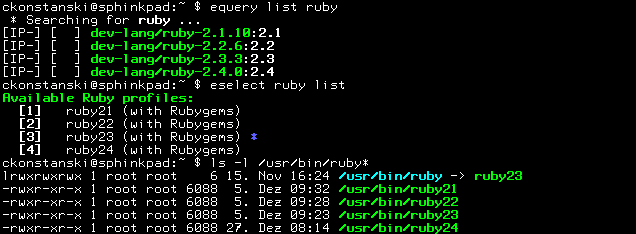
\includegraphics[scale=0.5]{eselect_1}
\end{frame}

\begin{frame}
  \frametitle{Ruby Version Management}

  There are systems similar to python's virtualenv that help manage
  the version problem by installing copies of ruby and libraries that
  are local to an application.

  \begin{itemize}
  \item rvm
  \item rbenv
  \item ruby-build
  \item chruby
  \item ruby-install
  \end{itemize}

  If you don't need to manage the ruby interpreter itself, but only
  need to manage the libraries on a per-application basis;

  \begin{itemize}
  \item rubygems
  \item bundler
  \end{itemize}
\end{frame}

\begin{frame}
  \frametitle{Running Ruby}
  \begin{itemize}
  \item Interactively via IRB
  \item Source code stored in files
  \end{itemize}
\end{frame}

\begin{frame}
  \frametitle{IRB}

  IRB is the interactive ruby shell. You can type ad-hoc ruby
  statements at the irb prompt and they will execute immediately. It
  is a great tool for iterative programming and for testing out new
  ideas.

  Here is a very simple example of an IRB session.

  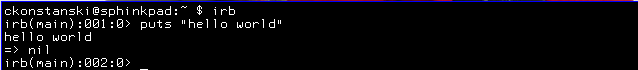
\includegraphics[scale=0.5]{irb_1}

  And here is a slightly more involved example which demonstrates that
  the environment saves the state that is created by the statements
  that you execute.

  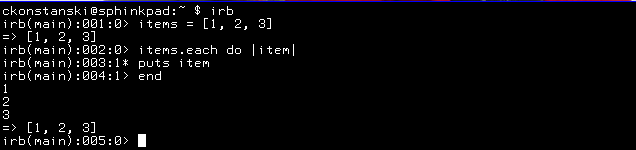
\includegraphics[scale=0.5]{irb_2}

  Type exit, quit or CTRL-d to exit an IRB session.
\end{frame}

\begin{frame}
  \frametitle{Source Files}

  Like all programming languages, you can create source files that
  contain the statements you wish to run. Ruby source files generally
  have an .rb extension.
  
  
  
\end{frame}

\end{document}
